\newpage
\section{Ciclomotor gasolina}
\label{anexo:Ciclomotor Gasolina}

Los \gls{ciclomotores} son vehículos que se han usado durante años para realizar el reparto a domicilio por su simplicidad, bajo coste y las prestaciones que ofrece para maniobras. Hoy en día, dado el desarrollo tecnológico y la reducción de costes en otros vehículos, el uso del ciclomotor ha disminuido, sin embargo, siguen siendo una referencia, en cuanto a reparto se refiere.

\begin{figure}[h]
    \centering
    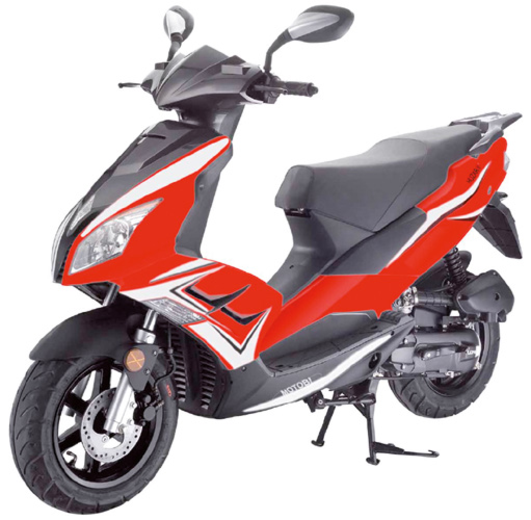
\includegraphics[scale = 1]{archivos/ciclomotor.pdf}
    \caption{Ciclomotor básico.}
    \label{fig:ciclomotor_basico}
\end{figure}

Al igual que otros vehículos, la \gls{dgt} recoge una serie de normas que deben cumplir todos los poseedores de un ciclomotor \cite{dgtciclomotores,boe11722}.

Las normas más destacables que influyen en la valoración de un modelo son las siguientes:
\begin{itemize}
    \item Está prohibido circular con el escape libre y emitir ruidos, gases u otros contaminantes.
    \item No podrán tener más luces y catadióptricos que los instalados por el fabricante.
    \item Los ciclomotores llevarán obligatoriamente un espejo retrovisor en el lado izquierdo. \textit{Opcionalmente, podrán llevar otro en el lado derecho.}
\end{itemize}

Acorde la normativa impuesta por la \gls{dgt} para matricular un ciclomotor, la tasa que corresponde es la 1.2 y asciende a 27,85 \glssymbol{euro}, esto quiere decir que al precio total de los ciclomotores hay que incluir el precio de la matriculación  \cite{dgtciclomotores}.


% El equipamiento que debe llevar el conductor de un ciclomotor es el siguiente:

% \begin{itemize}
%     \item Un casco, que debe estar homologado y correctamente abrochado. 
%     \item Chalecos u otros elementos reflectantes, ropas de color claro, casco con elementos reflectantes.
%     \item Sistema de alumbrado en perfectas condiciones con luces delanteras y traseras potentes, bien regladas y limpias.
% \end{itemize}



La \gls{itv} no contempla en su \textit{manual de modificaciones de vehículos} \cite{itvciclomotores} los cambios en la carrocería de los ciclomotores, por lo tanto, cualquier cambio de imagen para seguir la identidad corporativa de la empresa es de libre elección.

\subsection{Catálogo de modelos}
Después de una búsqueda exhaustiva de ciclomotores específicos para el reparto, se ha llegado a la conclusión de que los siguientes modelos satisfacen las necesidades expuestas anteriormente \cite{kymcofichatecnica, apriliafichatecnica, piaggiofichatecnica,peugeotfichatecnicars,peugeotfichatecnicaspeed,apriliasxr50,motormapfre}.
% kymcagility50
\begin{table}[h]
\resizebox{\textwidth}{!}{
\begin{tabular}{cccccccc}
\hline
\multicolumn{1}{|c|}{}                           & \multicolumn{1}{c|}{Precio {[}\gls{euro}{]}} & \multicolumn{1}{c|}{Homologación} & \multicolumn{1}{c|}{Cilindrada  {[}\gls{cc}{]}} & \multicolumn{1}{c|}{Consumo {[}\gls{litroporkilometro}{]}} & \multicolumn{1}{c|}{Depósito de gasolina {[}\gls{litros}{]}} & \multicolumn{1}{c|}{Emisiones \gls{dioxidodecarbono} {[}\gls{gramosporkilometros}{]}} & \multicolumn{1}{c|}{Peso {[}\gls{kg}{]}} \\ \hline
\multicolumn{1}{|c|}{KYMCO Agility Carry 50 E5}  & \multicolumn{1}{c|}{1.840,00}           & \multicolumn{1}{c|}{Euro 5}       & \multicolumn{1}{c|}{50}                   & \multicolumn{1}{c|}{2}                  & \multicolumn{1}{c|}{6}                            & \multicolumn{1}{c|}{47}                       & \multicolumn{1}{c|}{105}           \\ \hline
\multicolumn{1}{|c|}{Aprilia SXR 50}             & \multicolumn{1}{c|}{2.499,00}           & \multicolumn{1}{c|}{Euro 5}       & \multicolumn{1}{c|}{50}                   & \multicolumn{1}{c|}{2.5}                & \multicolumn{1}{c|}{7}                            & \multicolumn{1}{c|}{58}                       & \multicolumn{1}{c|}{100}           \\ \hline
\multicolumn{1}{|c|}{Liberty 50 Euro 5}          & \multicolumn{1}{c|}{2.499,00}           & \multicolumn{1}{c|}{Euro 3}       & \multicolumn{1}{c|}{49}                   & \multicolumn{1}{c|}{2.3}                & \multicolumn{1}{c|}{6}                            & \multicolumn{1}{c|}{48}                       & \multicolumn{1}{c|}{88}            \\ \hline
\multicolumn{1}{|c|}{Speedfight 50 4T EURO 5}    & \multicolumn{1}{c|}{2.990,00}           & \multicolumn{1}{c|}{L1e-B}        & \multicolumn{1}{c|}{50}                   & \multicolumn{1}{c|}{2.3}                & \multicolumn{1}{c|}{8}                            & \multicolumn{1}{c|}{51}                       & \multicolumn{1}{c|}{107}           \\ \hline
\multicolumn{1}{|c|}{Peugeot TWEET 50 RS EURO 5} & \multicolumn{1}{c|}{2.390,00}           & \multicolumn{1}{c|}{L1e-B}        & \multicolumn{1}{c|}{49}                   & \multicolumn{1}{c|}{2.4}                & \multicolumn{1}{c|}{5.4}                          & \multicolumn{1}{c|}{53}                       & \multicolumn{1}{c|}{100}           \\ \hline
                                                 &                                     &                                   &                                           &                                         &                                                   &                                               &                                   
\end{tabular}}
\caption{Comparación de distintos modelos de ciclomotores de reparto.}
\label{tab:comparacion de distintos modelos de ciclomotores de reparto}
\end{table}

La \autoref{tab:comparacion de distintos modelos de ciclomotores de reparto} recoge las principales características de diversas motos. Considerando la mejor relación calidad-precio, la mejor opción en cuanto al consumo, emisiones, depósito y peso, se ha llegado a la conclusión de que la moto más óptima para las condiciones que presenta la empresa es la \textbf{``KYMCO Agility Carry 50 E5''}.

La \textbf{``KYMCO Agility Carry 50 E5''}, es el modelo más barato de los cinco, se encuendra dentro de la categoría de vehículos L1, cuenta con una homologación \gls{euro5} \cite{euro5}, el mejor consumo respecto al resto, un depósito grande que permitirá recorrer largas distancias y las emisiones de \gls{dioxidodecarbono} son las más bajas, en contra parte el peso de la moto es elevado, pero que, comparado con otros modelos en el que la diferencia es de 2 \gls{kg} o 5 \gls{kg} y las prestaciones son menores, no tiene mucha importancia.

\newpage
% \addcontentsline{toc}{section}{Referencias}
% \section*{Referencias}
% \label{referencias_nucleo}
% \makeatletter
% \def\@bibitem#1{\item\if@filesw \immediate\write\@auxout
%   {\string\bibcite{#1}{A\the\value{\@listctr}}}\fi\ignorespaces}
% \def\@biblabel#1{[A{#1}]}
% \makeatother
% \printbibheading[title={Referencias},heading=bibintoc]
\nocite{*}
\newrefcontext[labelprefix=\thesection.]
\printbibheading[title={Referencias},heading=subbibintoc]
\printbibliography[heading=none,resetnumbers=true,keyword=ciclogasoref]
\newpage
